\documentclass[12pt]{article}

% margins and page style
\usepackage[margin=2.5cm]{geometry}
\usepackage{fancyhdr}
\pagestyle{fancy} 

% spaces between paragraphs
\usepackage[parfill]{parskip}

% fonts
\usepackage[T1]{fontenc}
\usepackage[scaled=0.92]{helvet}
\renewcommand*\familydefault{\sfdefault}

% font size of section headings
\usepackage{sectsty}
\sectionfont{\fontsize{14}{15}\selectfont}

% tables 
\usepackage{booktabs}
\renewcommand{\arraystretch}{1.5}

% figures
\usepackage{graphicx}
\usepackage[font=small,labelfont=bf]{caption} 

% colors
\usepackage[dvipsnames,svgnames,hyperref,table]{xcolor}

% symbols
\usepackage{gensymb}

% hyperlinks
\usepackage{hyperref}
\hypersetup{
  pdfauthor={Erin C. McKiernan},
  colorlinks=true,
  urlcolor=Bittersweet,
  linkcolor=blue,
  citecolor=Purple,
}

% bib options
\let\oldbibliography\thebibliography
\renewcommand{\thebibliography}[1]{\oldbibliography{#1}
\setlength{\itemsep}{0pt}} 
\usepackage[numbers,sort&compress]{natbib} 
\bibliographystyle{unsrtnat}


% title and authors
\usepackage{authblk}
\title{\vspace{-1.8cm}\Large{\textbf{Building a simple prosthetic hand that responds to myoelectric signals}}}
\author[1]{Daniel G\'omez P\'erez}
\author[2]{Erin C. McKiernan}
\affil[1]{\small{Licenciatura en F\'isica Biom\'edica, Facultad de Ciencias, Universidad Nacional Aut\'onoma de M\'exico}}
\affil[2]{\small{Departamento de F\'isica, Facultad de Ciencias, Universidad Nacional Aut\'onoma de M\'exico}}

\date{}

%%%%%%%%%%%%%%%%%%%%%%%%%%%%%%%%%%%%%%%%%%%%%%%%%%%%%%%%%%%%
 
\begin{document}
\maketitle


\section*{OVERVIEW}
In this laboratory practical, students will learn about the basic anatomy of the hand, and how the muscles and tendons of the hand work together to control its movement. Students will learn how to build a simple prosthetic hand from lightweight materials, how to connect this hand to a programmable interface, and how to control movement of the hand by feeding electromyographics signals from the bicep muscle through the interface. Overall, this practical will help students to better understand the biomechanics of one part of the musculoskeletal system, the instrumentation of simple prosthetics, and the relationship between electrical signals and movement. 

\section*{SPECIFICATIONS}
\begin{tabular}{p{6cm} p{10cm}}
\textbf{Level of study:} & Undergraduate \\
\textbf{Degree programs:} & Biology, Physics, Biomedical Physics, others \\
\textbf{Semester:} & 4-6th (i.e., 2nd-3rd year undergrads) \\ 
\textbf{For use in courses:} & Systems Physiology, others \\
\textbf{Recommended prior courses:} & Molecular \& Cellular Biology \\
\textbf{Prerequisite practicals:} & Electromyography Basics \\
\textbf{Duration of practical:} & multiple sessions \\
\textbf{Setting:} & Classroom or laboratory \\
\textbf{Safety considerations:} & None \\
\textbf{Other indications:} & Wear loose clothing to permit electrode placement
\end{tabular}

\section*{OBJECTIVES}
\textbf{Before doing this lab you should be able to:}
\begin{itemize}
\item understand the basics of muscle contraction and biomechanics of skeletal muscles
\item understand the basics of electromyography (EMG) signal production 
\item know the basic anatomy of the hand, including the key muscles and tendons 
\end{itemize}
 
\vspace{0.3cm}

\textbf{In this lab you will:}
\begin{itemize}
\item learn how to construct a simple prosthetic hand
\item arrange string 'tendons' on the hand to permit finger movements
\item 
\item 
\end{itemize}

\vspace{0.3cm}
 
\textbf{After doing this lab you should be able to:}
\begin{itemize}
\item describe the basic concepts underlying myographic prostheses
\item 
\item design several ways to improve the prosthetic hand by using different materials, different ways to arrange the 'tendons', etc.
\end{itemize}

\section*{EQUIPMENT}

 \begin{itemize}
	\item Muscle SpikerShield (Backyard Brains)
    \item 3 surface electrodes (Backyard Brains or other provider)
    \item orange cable with alligator clips to connect electrodes to SpikerShield (Backyard Brains)
    \item cable to connect SpikerBox to a computer (Backyard Brains)
 	\item cardboard, or other lightweight material that can be easily cut into shape and is flexible enough to move
 	\item at least 5 heavy-duty threads, each approximately 30 cm long 
 	\item staples and stapler
 	\item motor? type?
\end{itemize}

\section*{BACKGROUND}

\subsection*{Bones and joints of the human hand}
The human hand has a complex skeletal structure, comprising 27 individual bones \citep{kumar2009hand,panchal2013skeletal} (Fig. \ref{fig:bonesJoints}). Starting proximally, at the base of the hand, we have the 8 carpal bones which make up the wrist. Morphologically, the carpal bones are classified as short bones, with cuboid-like appearance \citep{openStaxBones}. Short bones allow for some movement, but are more for structural support. Moving distally, we find the 5 metacarpal bones, which run through the palm area of the hand. Metacarpal bones are classified as long bones, and their primary function is to connect the wrist to the fingers. More distally still, we have the 14 phalanges, also classified as long bones and divided into the proximal, intermediate, and distal phalanges. Note that the thumb is the only digit which does not have an intermediate phalanx. Articulations of the different phalanges allow for gross motor movements such as grasping, as well as fine motor movements like playing the piano or threading a needle \citep{duncan2013biomechanics},.

\begin{figure}[h!]
\centering
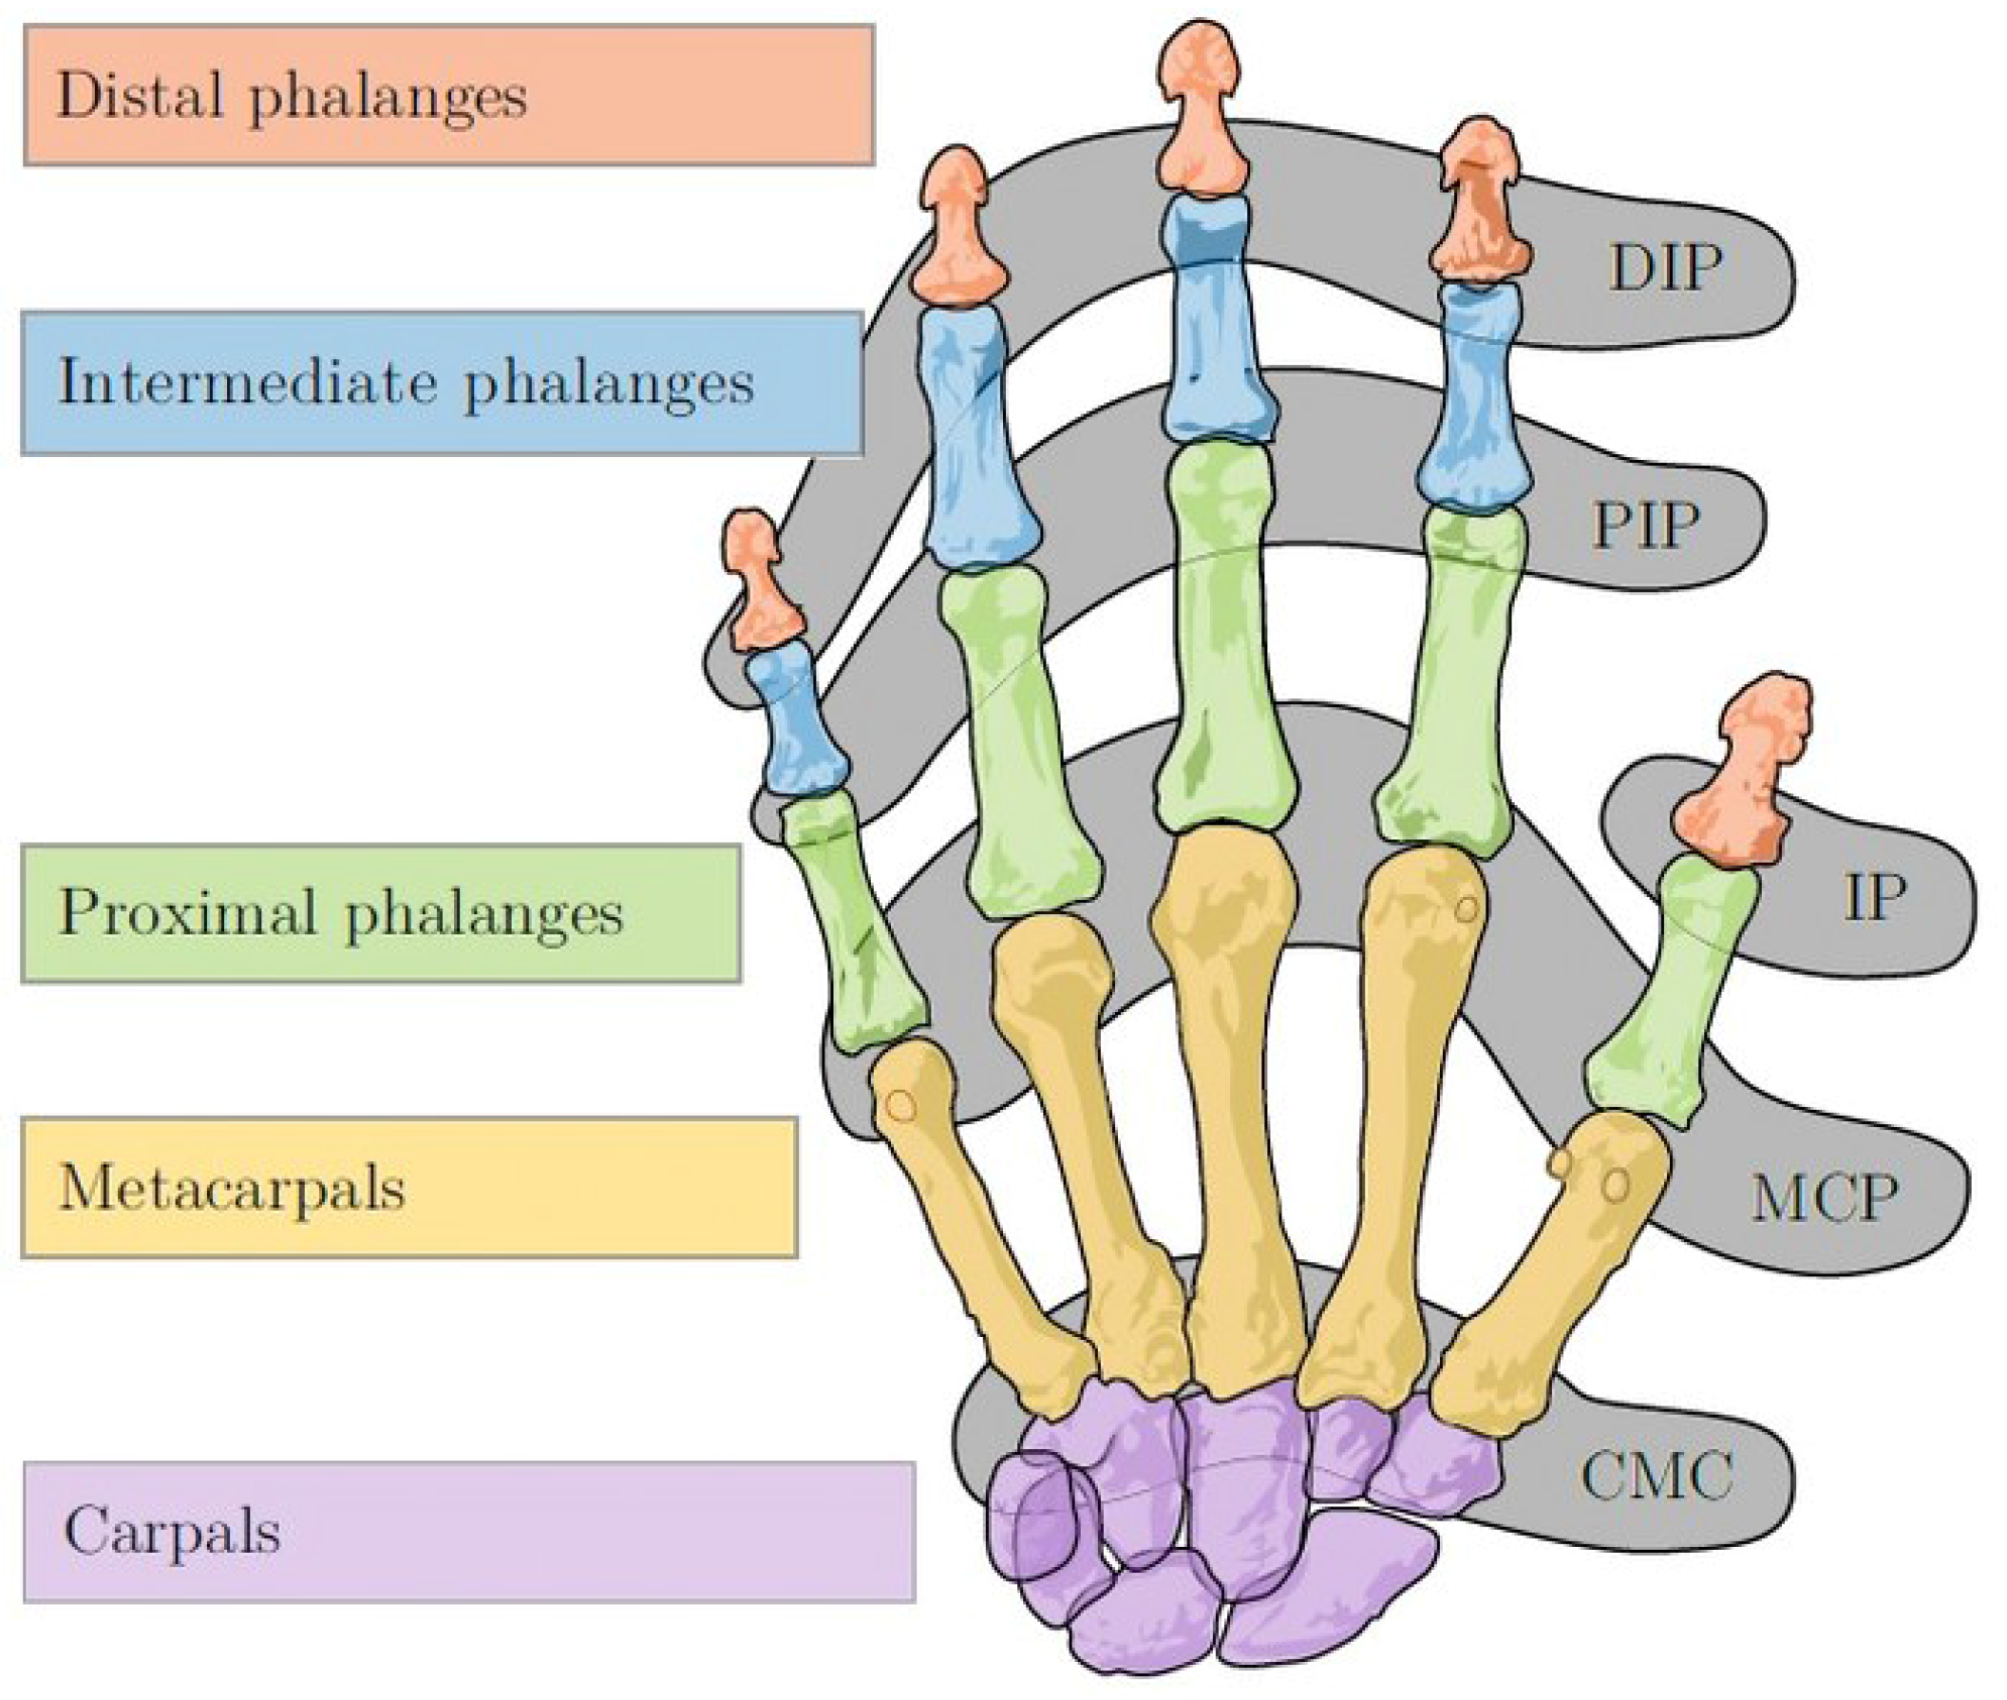
\includegraphics[width=0.8\textwidth]{images/bones_joints_hand.png}
\caption{Bones and joints in the human hand. Image credit: Tavakoli \textit{et al.}, 2016 \citep{tavakoli2016uc}, CC BY 4.0.}
\label{fig:bonesJoints}
\end{figure}

Joints form where the different bones in the hand meet \citep{tortora2014principles} (Fig. \ref{fig:bonesJoints}). The meeting points between the carpal and metacarpal bones are called the carpometacarpal (CMC) joints \citep{ombregt2013applied,panchal2013skeletal}. These joints allow for movements like flexion, extension, and rotation of the hand. Where the proximal metacarpals and phalanges meet are known as the metacarpophalangeal (MCP) joints. The proximal interphalangeal (PIP) joints are where the proximal and intermediate phalanges meet. These joints allow you to bend (flex) your fingers at their midpoint. Both the MCP and PIP joints are important in actions such as forming a fist and gripping, and also participate in fine motor movements \citep{duncan2013biomechanics}. Finally, where the intermediate and distal phalanges meet are the distal interphalangeal (DIP) joints. The DIP joints have much more restricted movement compared to the MCP and PIP joints, but do allow some flexion. Note that because the thumb lacks an intermediate phalanx \citep{panchal2013skeletal}, it only has an interphalangeal (IP) joint where the proximal and distal phalanges meet (Fig. \ref{fig:bonesJoints}).

\subsection*{Muscles of the hand}

The force required to move the bones of the hand is provided by skeletal muscles. These muscles can be divided into two main groups, those intrinsic and those extrinsic to the hand \citep{openStaxMuscles,tortora2014principles,ombregt2013applied}. 

\subsubsection*{Intrinsic muscles of the hand}

The intrinic muscles both arise from and terminate in the hand \citep{openStaxMuscles,tortora2014principles,ombregt2013applied,schreuders2007intrinsic} (Fig. \ref{fig:intMuscles}). They are classified into groups based on anatomical location and function.

\underline{Thenar muscles}: 
\begin{itemize}
    \item \textit{abductor pollicis brevis}: abduction of the thumb (first digit) at the CMC joint, moving it away from the palm at a {90\degree} angle; participates in opposition and flexion of the thumb
    \item \textit{adductor pollicis}: adduction of the thumb at the CMC joint, moving it back towards the palm
    \item \textit{opponens pollicis}: flexion of the thumb at the CMC joint to produce opposition, where the thumb comes into contact with the other fingers
    \item \textit{flexor pollicis brevis}: flexion of the thumb at the MCP joint
\end{itemize}

\underline{Hypothenar muscles}: 
\begin{itemize}
    \item \textit{abductor digiti minimi}: abduction of the little finger (fifth digit) at the MCP joint, moving it away from the ring finger (fourth digit)
    \item \textit{flexor digiti minimi brevis}: flexion of the little finger at the MCP joint
    \item \textit{opponens digiti minimi}: flexion and rotation of the little finger at the CMC joint to bring it into contact (opposition) with the thumb
\end{itemize}   

\underline{Interosseous muscles}: 
\begin{itemize}
    \item \textit{dorsal interossei}: abduction of the digits, spreading the fingers out and away from the midline; participate in flexion of the MCP joints and extension of the PIP and DIP joints 
    \item \textit{palmar interossei}: adduction of the digits, bringing the fingers toward the midline; participate in flexion of the MCP joints and extension of the PIP and DIP joints 
\end{itemize}

\underline{Lumbricalis muscles}:
\begin{itemize}
    \item \textit{I, II, III, IV}: together with the interosseous muscles, all four muscles participate in flexion of the MCP joints and extension of the IP joints of the 2nd through 5th digits, respectively 
\end{itemize}

\begin{figure}[h!]
\centering
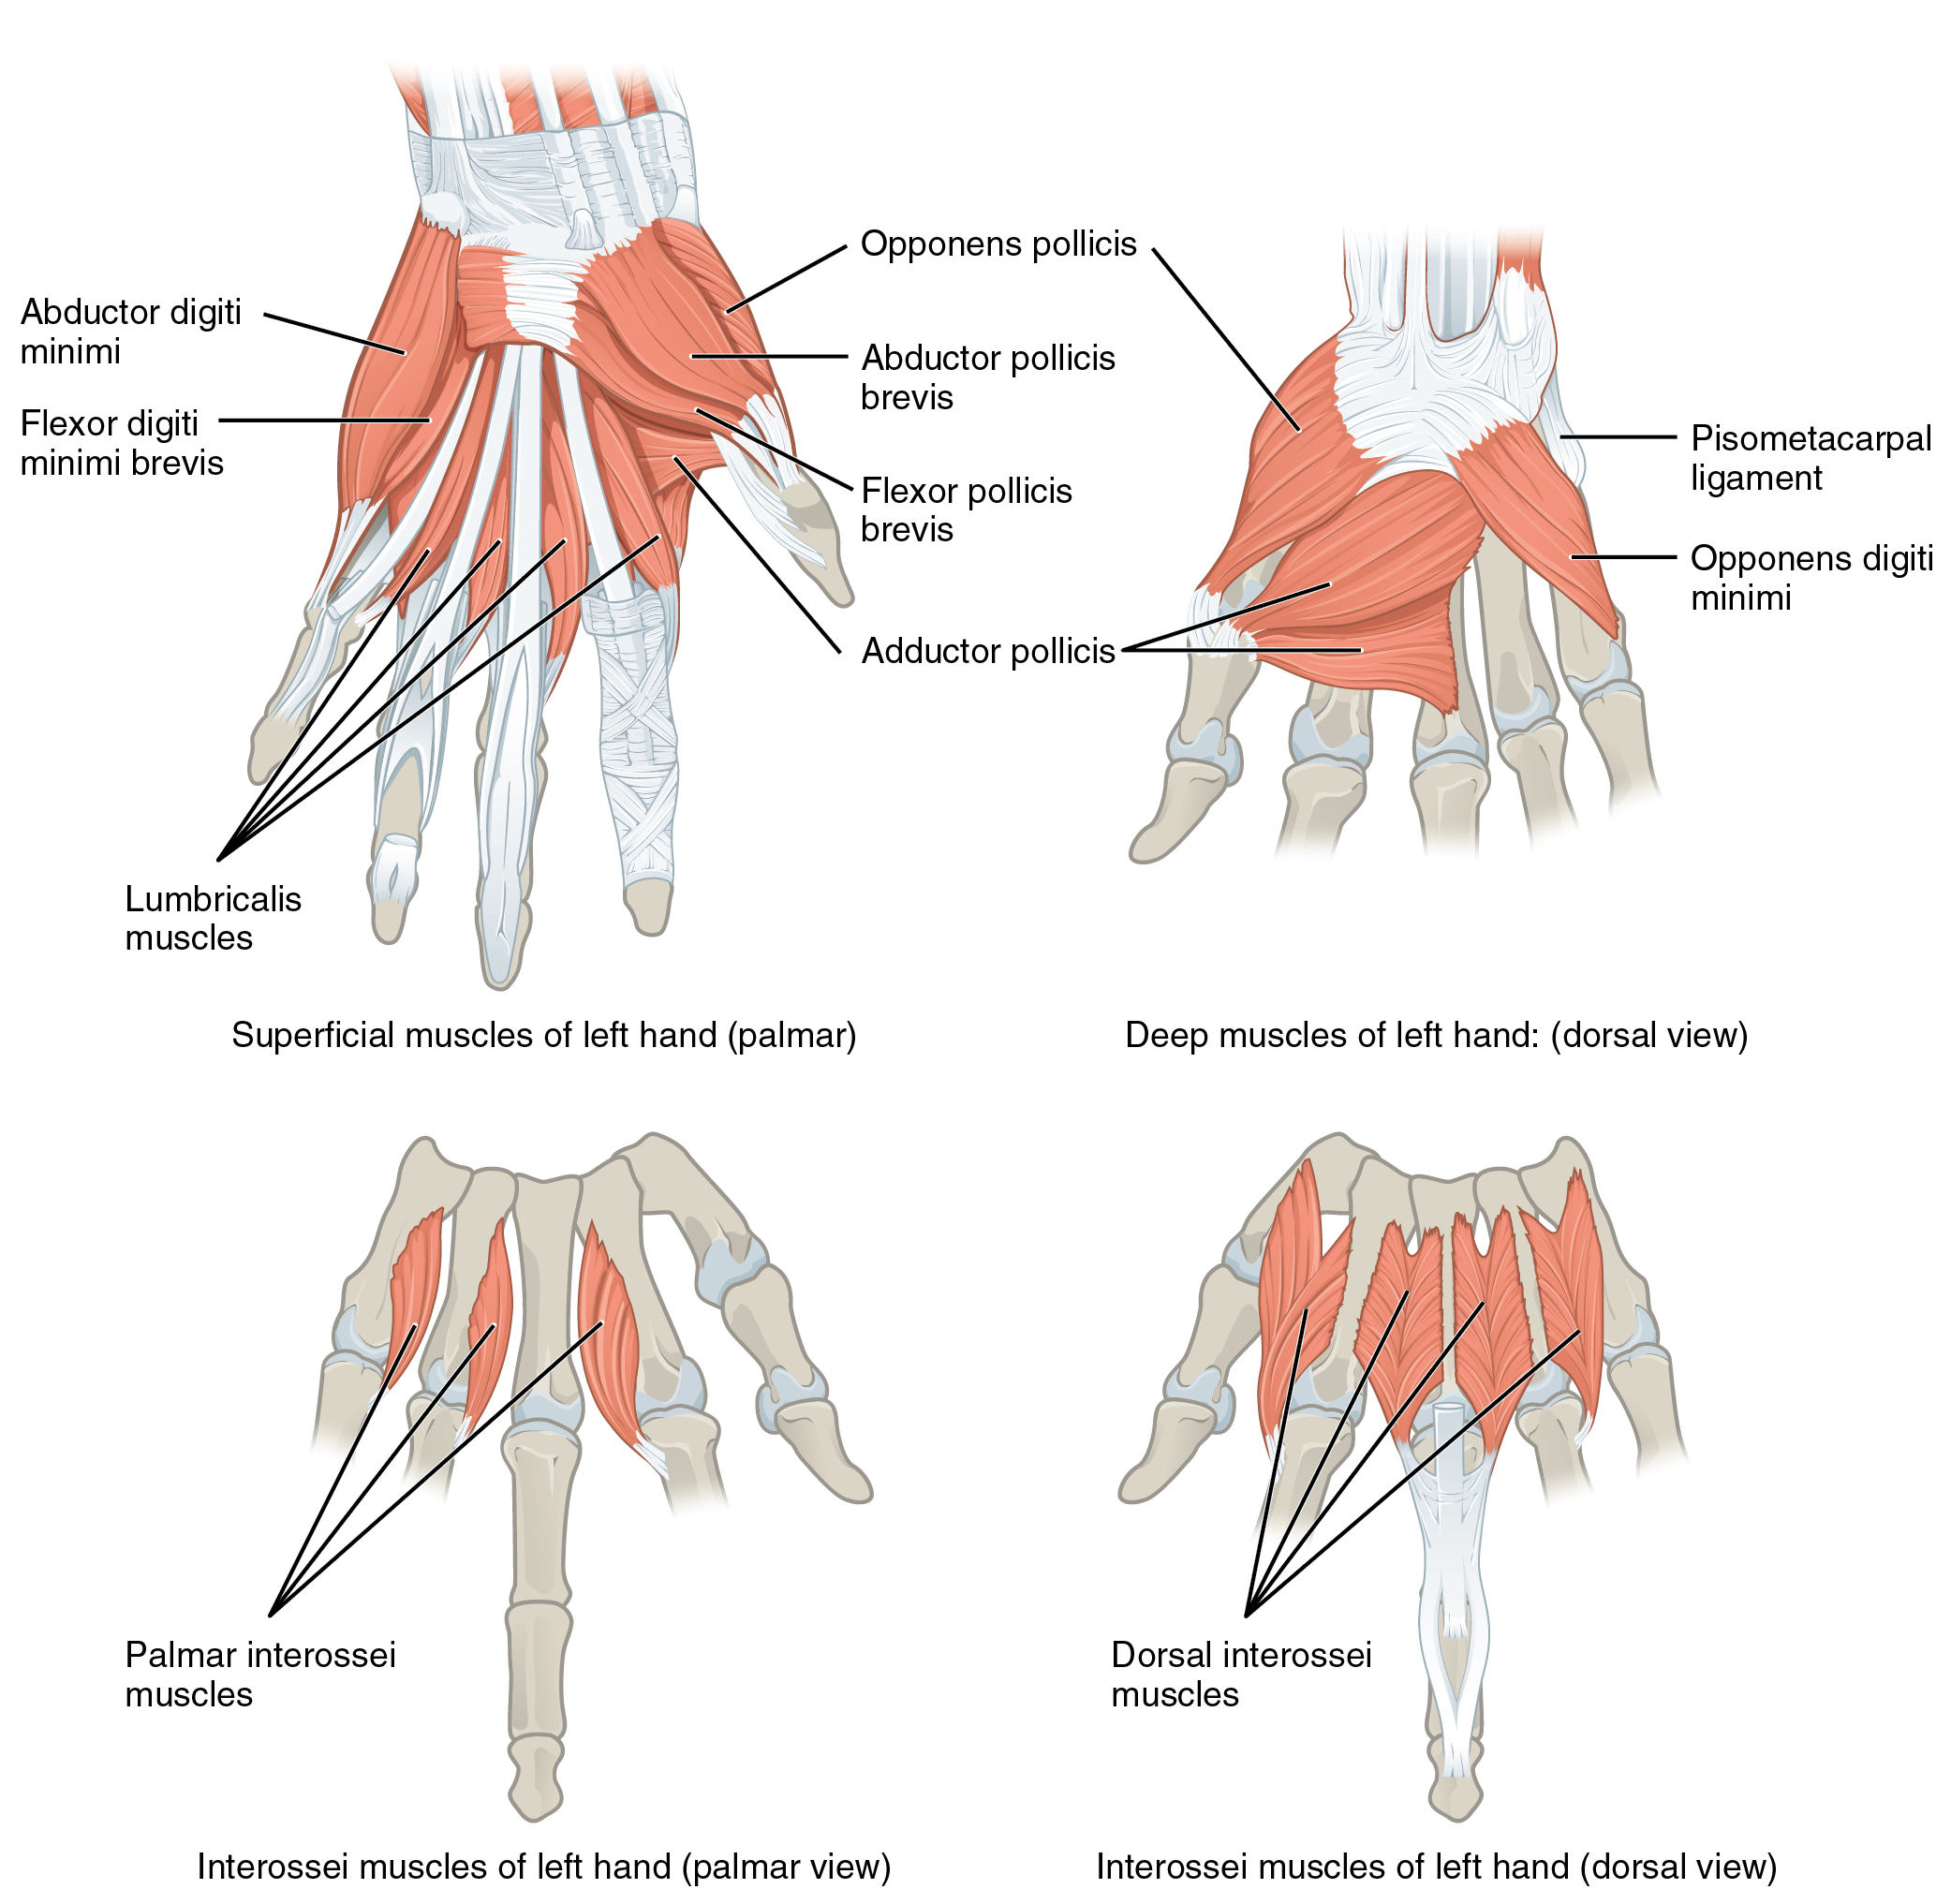
\includegraphics[width=0.95\textwidth]{images/Intrinsic_Muscles_of_the_Hand.jpg}
\caption{Intrinsic muscles of the hand. Image credit: OpenStax \citep{openStaxMuscles}, CC BY 4.0.}
\label{fig:intMuscles}
\end{figure}

\subsubsection*{External muscles of the hand}

The external muscles are those which originate outside the hand, primarily in the forearm, but insert into the hand \citep{openStaxMuscles,tortora2014principles,ombregt2013applied} (Fig. \ref{fig:extMuscles}). 

The \underline{extrinsic flexors} include: 
\begin{itemize}
    \item \textit{flexor carpi ulnaris}: flexion and adduction of the hand at the wrist
    \item \textit{palmaris longus}: aids in flexion of the hand at the wrist
    \item \textit{flexor carpi radialis}: flexion and abduction of the hand at the wrist
    \item \textit{flexor digitorum superficialis}: flexion of the 2nd to 5th digits at the PIP and MCP joints (after flexion is initiated)
    %\item \textit{pronator teres}: pronation to turn the palm of the hand downwards; aids in elbow flexion
    \item \textit{flexor digitorum profundus}: flexion of the 2nd to 5th digits at the DIP, PIP, and MCP joints (after flexion is initiated)
    \item \textit{flexor pollicis longus}: flexion of the thumb at the IP and MCP joints
    %\item \textit{pronator quadratus}: aids in pronation of the hand
\end{itemize}

The \underline{extrinsic extensors} include: 
\begin{itemize}
    \item \textit{extensor carpi radialis longus}: extension and abduction of the hand at the wrist
    \item \textit{extensor carpi radialis brevis}: extension and abduction of the hand at the wrist
    \item \textit{extensor digitorum}: extension of 2nd to 5th digits at the MCP and IP joints; wrist extension
    \item \textit{extensor digiti minimi}: extension of the little finger (5th digit) at the MCP and PIP joints
    \item \textit{extensor carpi ulnaris}: extends and adducts the hand at the wrist
    \item \textit{abductor pollicis longus}: abduction of the thumb and extension at the CMC joint
    \item \textit{extensor pollicis brevis}: extension of the thumb at the MCP joint
    \item \textit{extensor pollicis longus}: extension of the thumb at the CMC and IP joints
    \item \textit{extensor indicis}: extension of the index finger (2nd digit) at all joints
\end{itemize}

\begin{figure}[h!]
\centering
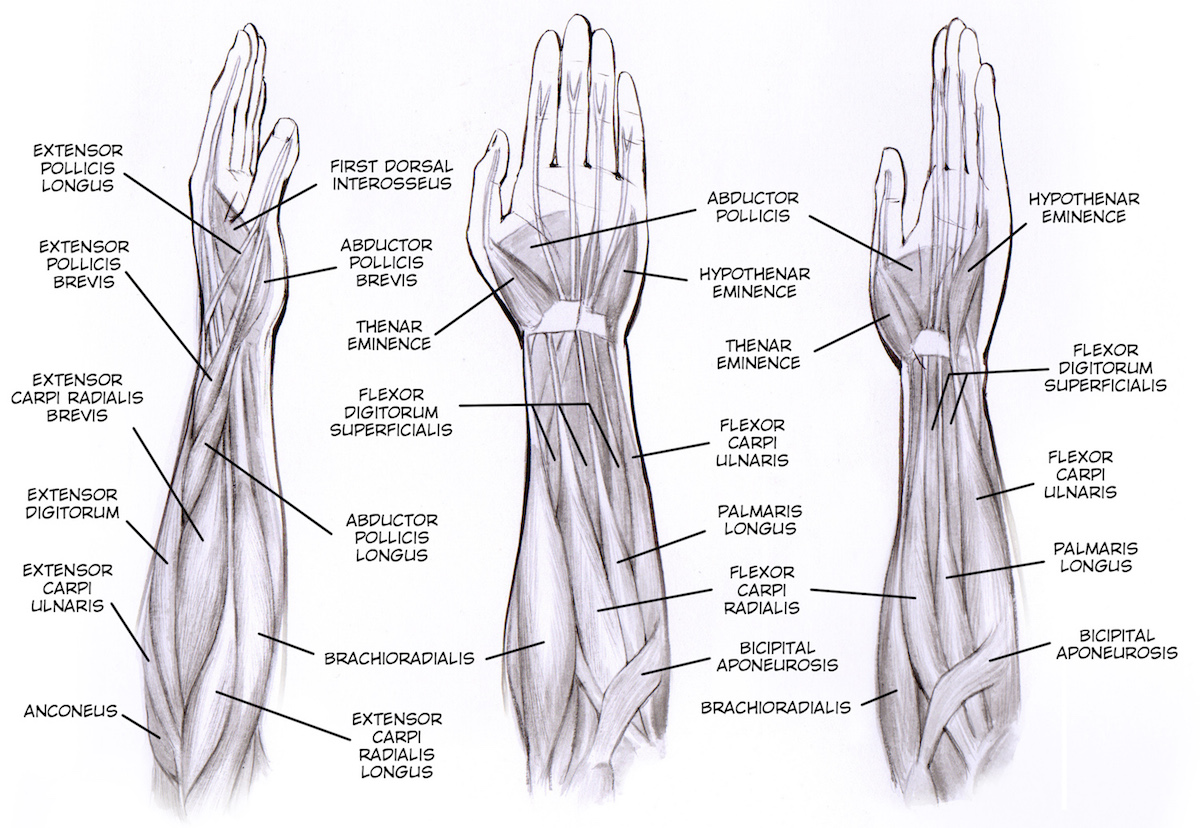
\includegraphics[width=0.95\textwidth]{images/muscles_of_hand.jpg}
\caption{Some of the intrinsic and extrinsic muscles of the hand. Image credit: Backyard Brains \citep{backyardBrainsHand}, CC BY-SA 3.0.}
\label{fig:extMuscles}
\end{figure}

\subsection*{Tendons of the hand}  
Tendons are collagenous fibers that connect muscles to bone \citep{tortora2014principles}. When a muscle contraction occurs, the force generated is transmitted to the bones via the tendons \citep{kirkendall1997function}. We can think of these tendons like cords; depending on where the cords insert, pulling on them will produce movement at different joints. 
Since they extend from the muscle, the corresponding tendons bear the same name as the muscle itself. Therefore, as we did with the muscles, we can classify the tendons based on whether they participate in flexion (bending) or extension (straightening). While in the previous section we looked at several different flexors and extensors, here we focus only on tendons that flex or extend the fingers.

\subsubsection*{Finger flexors}
The finger flexors run along the palmar side of the hand (Fig. \ref{fig:tendons}), and include the flexor digitorum supercialis (FDS), flexor digitorum profundus (FDP), and flexor pollicis longus (FPL) tendons \citep{tortora2014principles,ombregt2013applied}. All of these tendons extend from extrinsic muscles that originate in the forearm. Flexion of the 2nd through 5th digits is controlled by the FDS and FDP tendons, which insert at the base of the middle and distal phalanges, respectively. Additionally, two groups of intrinsic muscles aid in flexion of the 2nd to 5th digits: the lumbricalis and the interosseous muscles. The interosseous muscles have a double tendon, the short part of which inserts into the base of the proximal phalanges to aid in flexion of the MCP joints \citep{videoAtlas}. The lumbricalis muscles do not directly insert into bone, but instead insert into the FDP tendons and aid in flexion of the MCP joints \citep{valenzuela2018lumbricals}. The 1st digit (the thumb) is innervated by the FPL tendon. The thumb also has an additional flexor tendon, the flexor pollicis brevis (FPB), which extends from the intrinsic thenar muscle of the same name. Similarly, the 5th digit (the little finger) has an additional flexor tendon, the flexor digiti minimi brevis \citep{tortora2014principles}.

\subsubsection*{Finger extensors}
The finger extensors run along the dorsal side of the hand (Fig. \ref{fig:tendons}), and include the extensor digitorum communis (EDC), extensor digitorum minimi (EDM), extensor indicis proprius (EIP), extensor pollicis longus (EPL), and extensor pollicis brevis (EPB) tendons \citep{tortora2014principles,ombregt2013applied}. All of these tendons extend from extrinsic muscles that originate in the forearm. Extension of the 2nd through 5th digits is controlled by EDC tendons, which insert into the extensor expansion of the middle and distal phalanges. Extension is also controlled in the 5th digit by the EDM tendon, in the 2nd digit by the EIP tendon, and in the 1st digit by both the EPL and EPB tendons. Additionally, the long part of the interosseous double tendon and the lumbricals insert into the extensor expansion to aid in extension of the IP joints \citep{videoAtlas,ombregt2013applied}.

\begin{figure}[h!]
\centering
\begin{minipage}{.5\textwidth}
\centering
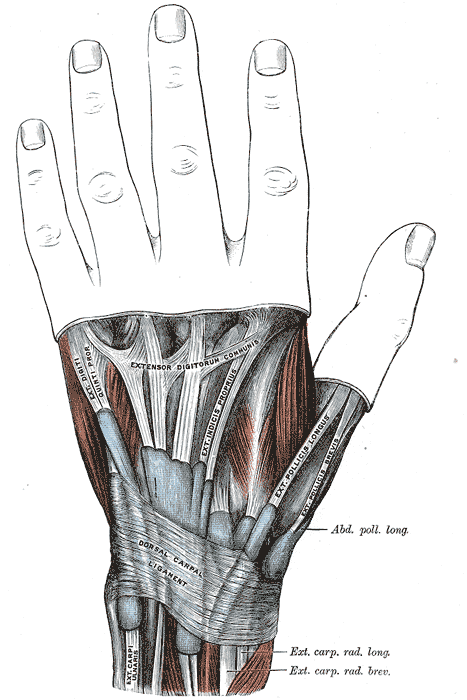
\includegraphics[width=0.83\textwidth]{images/gray_tendons_dorsal.png}
\end{minipage}%
\begin{minipage}{.5\textwidth}
\centering
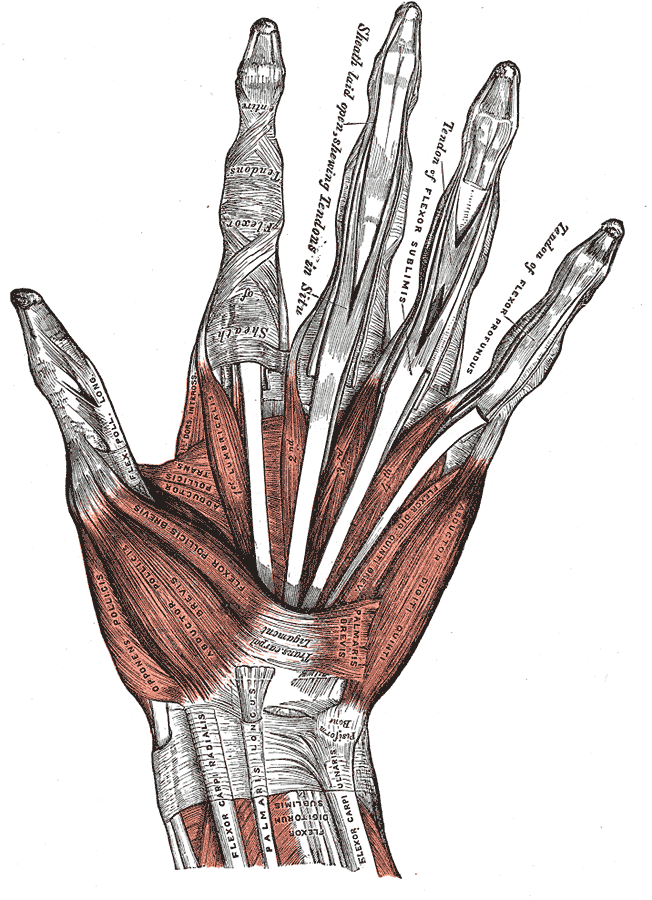
\includegraphics[width=0.9\textwidth]{images/gray_tendons_ventral.png}
\end{minipage}
\vspace{0.2cm}
%\begin{minipage}{.5\textwidth}
\centering
%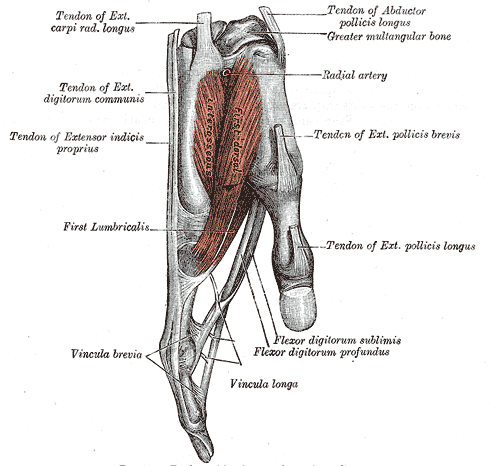
\includegraphics[width=0.9\textwidth]{images/Gray416.png}
%\end{minipage}%
%\begin{minipage}{.5\textwidth}
\centering
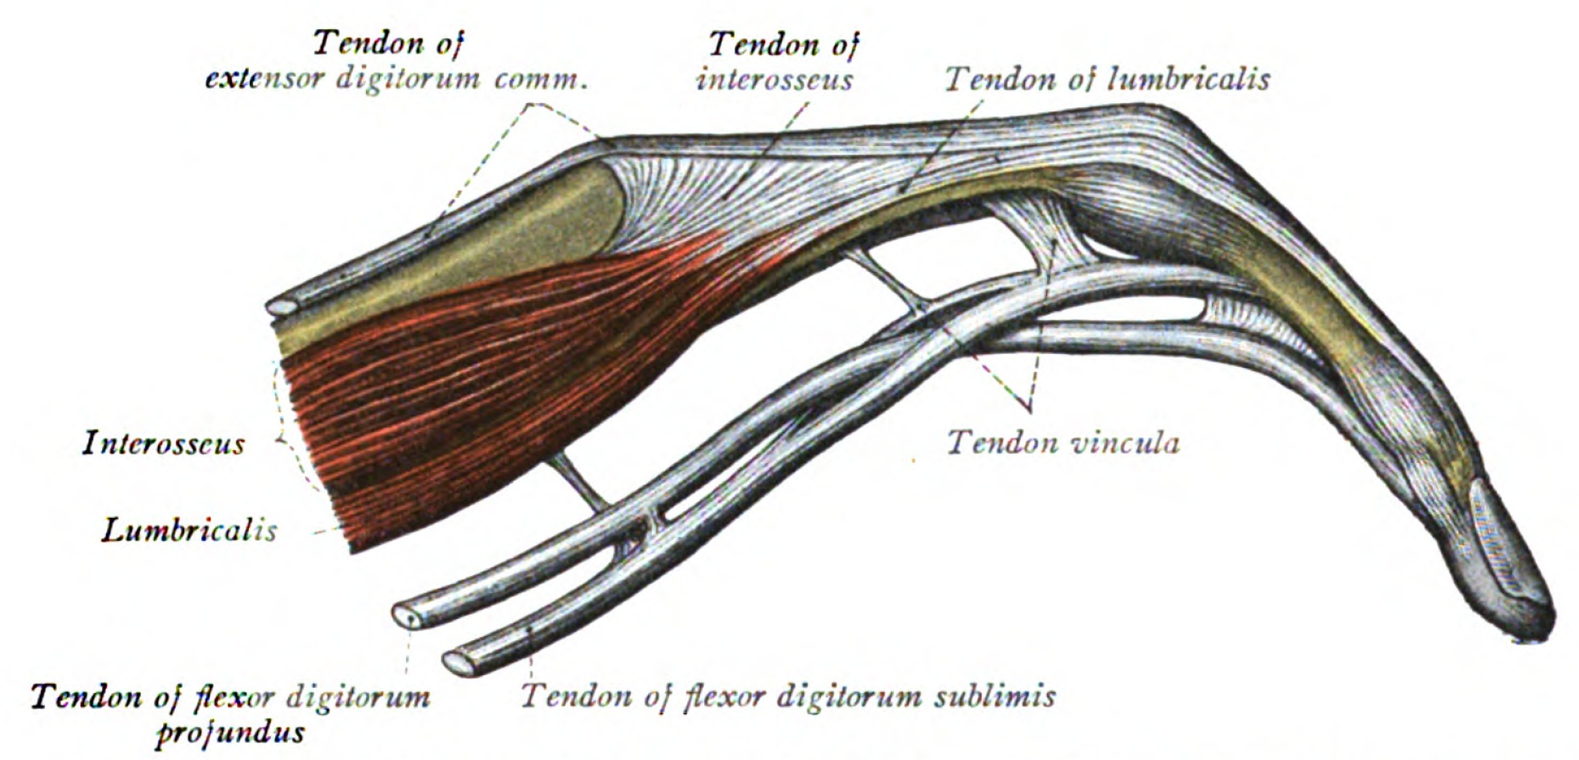
\includegraphics[width=0.65\textwidth]{images/extensorFlexor.png}
%\end{minipage}
\caption{Tendons of the hand. Dorsal (top left) and palmar (top right) views. From Gray's Anatomy, via Wikimedia Commons, Public Domain. \textit{Bottom center}: Drawing of a single finger, showing specific extensor and flexor tendons. Image credit: Sobotta's Atlas and Text-book of Human Anatomy 1909, via Wikimedia Commons, Public Domain.}
\label{fig:tendons}
\end{figure}

\subsection*{Myoelectric hand prostheses}
Every year, thousands of people worldwide undergo amputation of the upper limbs due to trauma, cardiovascular complications, and disease, among other causes. In the U.S. alone, it is estimated that as of 2005 around 1.6 million people were living with limb loss, of which over 500,000 were designated as loss of an upper limb including hands and fingers. These numbers are projected to double by the year 2050 \citep{ziegler2008estimating}. 

For those living with a loss of limb, a prosthesis (artificial limb) can be a great way to regain function and independence. There exist different types of prostheses, ranging from simply aesthetic to varying degress of functionality \citep{maat2018passive,ten20173d}. Some of the most promising are myoelectric prostheses, which use electromyogram signals recorded from skeletal muscles to control movements of the artificial limb \citep{geethanjali2016myoelectric}. The basic 


\subsection*{Study questions:}

\begin{enumerate}
    \item On which side of the prosthetic hand do you need to place the threads if you want them to act as finger flexor/extensor tendons?
    \item Where should you fix the threads if you want them to flex/extend the MCP, PIP, or DIP joints?
    \item Will you be able to accomplish individual control of the fingers and their different joints? If not, why? If so, how?
\end{enumerate}

\section*{PROCEDURE}

Before beginning, make sure you have all the necessary equipment and have installed the Backyard Brains recording software on your computer or smartphone. The following steps will guide you in setting up the equipment and carrying out recordings.

\subsection*{1. Construct the lightweight hand with `tendons'}

\vspace{0.2cm}

\begin{enumerate}
\item On a 20 x 30 cm rectangular piece of cardboard trace your hand, wrist, and part of the forearm with a pencil or pen.
\item Used the traced shaped as a guide, cut out the cardboard hand, and label one side 'dorsal' and the other side 'palmar'; save the extra cardboard for later
\item On the palmar side, draw horizontal lines on the fingers where the major MCP, DIP, and IP joints would be located and then gently bend the cardboard toward the palm at those points
\item  Cut five pieces of thread of 30 cm each and tape or glue one end of each thread to each of the distal fingertips
\item Once each thread is fixed at the tip, run the threads down each corresponding finger on the palmar as if they were large, single tendons and staple the threads down where each joint is marked
\item Staple at the base??
\item Depending on the consistency of the cardboard, the hand may need reinforcement in key places; if so, use the remaining cardboard and cut 5 rectangular strips slightly less than the width and length of each finger and a larger rectangle about the size of the palm
\item Glue the strips to the dorsal side of each finger and the larger rectangle to the dorsal side of the hand to reinforce the structure
\end{enumerate}
 
\subsection*{2. Connect the motor}

\begin{enumerate}
\item At the base of the cardboard forearm, cut a rectangular hole with the dimensiones of the servomotor, model MG995 (dimensions?)
\item Fix the motor in place using silicon glue and glue gun
\item Run the loose end of each thread down to the base of the hand and connect them to the motor; leave some but not too much slack in the threads, readjust as needed
\item Connect the cables on the motor to the EMG SpikerShield?
\end{enumerate}

\subsection*{3. Program the interface}

\begin{enumerate}
\item Connect the EMG SpikerShield to your computer using the blue USB cable
\item Open the Arduino software (free download at \href{https://www.arduino.cc/en/Main/software}{https://www.arduino.cc/en/Main/software})
\item From the 'Tools' menu, select the board Arduino Uno and the port in which the device is connected to the computer 
\item In the terminal, write the code that will be used to configure the interface and allow it to transmit electrical signals generated in the muscle to move the servomotor (see ref? or appendix for full code)
\item Once the code is written, compile it and upload it to the Arduino. If there are any errors in the code, it will not upload and may require debuggin
\end{enumerate}

\subsection*{4. Set up EMG recordings}

\begin{enumerate}
\item Place two surface electrodes a few centimeters apart and aligned in parallel with the muscle fibers of the bicep muscle
\item Place the ground electrode on the back of the hand
\item Take the orange cable and connect each of the red alligator clips to the recording electrodes on the bicep and the black alligator clip to the ground electrode
\item If necessary, EMG recording can be tested using the EMG SpikerBox and a smartphone (see practical ref?) 
\end{enumerate}

\subsection*{}

\subsection*{Potential modifications to the practical}

\begin{itemize}
    \item design hand to have both flexors and extensors (current model only has flexors and extension is passive)
\end{itemize}

\section*{ACKNOWLEDGMENTS}
This work was
supported by the Dirección General de Asuntos del Personal Académico, Programa de Apoyo a Proyectos para la Innovación y Mejoramiento de la Enseñanza at the Universidad Nacional
Autónoma de México (UNAM-DGAPA-PAPIME clave PE213817).
 
% BIBLIOGRAPHY
\begin{small}
\bibliography{refs}
\end{small}

\end{document}
